\documentclass[aspectratio=169]{beamer}

\usetheme{Madrid}
\usecolortheme{default}

\usepackage{listings}
\usepackage{booktabs}
\usepackage{hyperref}
\usepackage{xcolor}
\usepackage{array}
\usepackage{graphicx}
\usepackage{tcolorbox}
\usepackage{tikz}

% Code listing style
\lstset{
    basicstyle=\ttfamily\small,
    breaklines=true,
    backgroundcolor=\color{gray!10},
    keywordstyle=\color{blue},
    commentstyle=\color{green!50!black},
    stringstyle=\color{red!70!black},
    showstringspaces=false
}

% Conversation box styles for demo slides
\newtcolorbox{userbox}{
    colback=gray!15,
    colframe=gray!40,
    fonttitle=\bfseries\small,
    title=USER,
    boxrule=0.5pt,
    arc=2pt,
    left=4pt, right=4pt, top=2pt, bottom=2pt
}

\newtcolorbox{assistantbox}{
    colback=blue!5,
    colframe=blue!30,
    fonttitle=\bfseries\small,
    title=ASSISTANT,
    boxrule=0.5pt,
    arc=2pt,
    left=4pt, right=4pt, top=2pt, bottom=2pt
}

\title{Running Your Own AI}
\subtitle{D-Lab AI Pulse Workshop}
\author[D-Lab]{Materials: \url{https://github.com/dlab-berkeley/AI_Pulse}\\Feedback form: \url{https://forms.gle/x8KfejgCViE7t6iQA}}
\date{}

\begin{document}

% ===== SLIDE 1: Title =====
\begin{frame}[plain]
    \titlepage
\end{frame}

% =============================================================================
% OPENING (Slides 2-3)
% =============================================================================

% ===== SLIDE 2: Motivation =====
\begin{frame}{Why Run Your Own LLM?}
    \textbf{Why you might want to:}
    \begin{itemize}
        \vspace{0.3em}
        \item \textbf{Privacy:} Data never leaves your machine
        \vspace{0.3em}
        \item \textbf{Cost:} No API fees, no subscriptions
        \vspace{0.3em}
        \item \textbf{Customization:} Fine-tune to your needs
    \end{itemize}

    \vspace{0.8em}
    \textbf{Why you might not:}
    \begin{itemize}
        \vspace{0.3em}
        \item \textbf{Quality:} Smaller models, less capable
        \vspace{0.3em}
        \item \textbf{Setup:} More technical than a chat interface
        \vspace{0.3em}
        \item \textbf{Hardware:} Needs decent RAM/GPU for larger models
    \end{itemize}
\end{frame}

% ===== SLIDE 3: Roadmap =====
\begin{frame}{Roadmap}
    Today's application: using AI to help write a physics paper.

    \vspace{0.3em}
    Not every task needs a frontier model. Smaller models have their own advantages.

    \vspace{1em}
    \begin{enumerate}
        \vspace{0.3em}
        \item \textbf{Run it:} Ollama
        \vspace{0.3em}
        \item \textbf{Fit your paper in it:} context windows \& quantization
        \vspace{0.3em}
        \item \textbf{Make it yours:} LoRA fine-tuning on NRP
        \vspace{0.3em}
        \item \textbf{Share it:} Hugging Face deployment
    \end{enumerate}

    \vspace{1em}
    But first: 3 slides on how LLMs work, so that fine-tuning makes sense when we get there. Bear with me.
\end{frame}

% =============================================================================
% ACT 1: WHAT IS AN LLM? (Slides 4-8)
% =============================================================================

% ===== SLIDE 4: What is an LLM? =====
\begin{frame}{What is an LLM?}
    \begin{columns}[T]
        \begin{column}{0.42\textwidth}
            \begin{itemize}
                \vspace{0.3em}
                \item LLMs are a type of neural network.
                \vspace{0.3em}
                \item Neural networks are made of layers.
                \vspace{0.3em}
                \item Learning from raw data (pixels) is very hard.
                \vspace{0.3em}
                \item Each layer models increasingly abstract features: edges, contours, object parts, identity.
                \vspace{0.3em}
                \item \textbf{Parameters:} the total count of numbers across all layers. More layers, more parameters.
            \end{itemize}
        \end{column}
        \begin{column}{0.55\textwidth}
            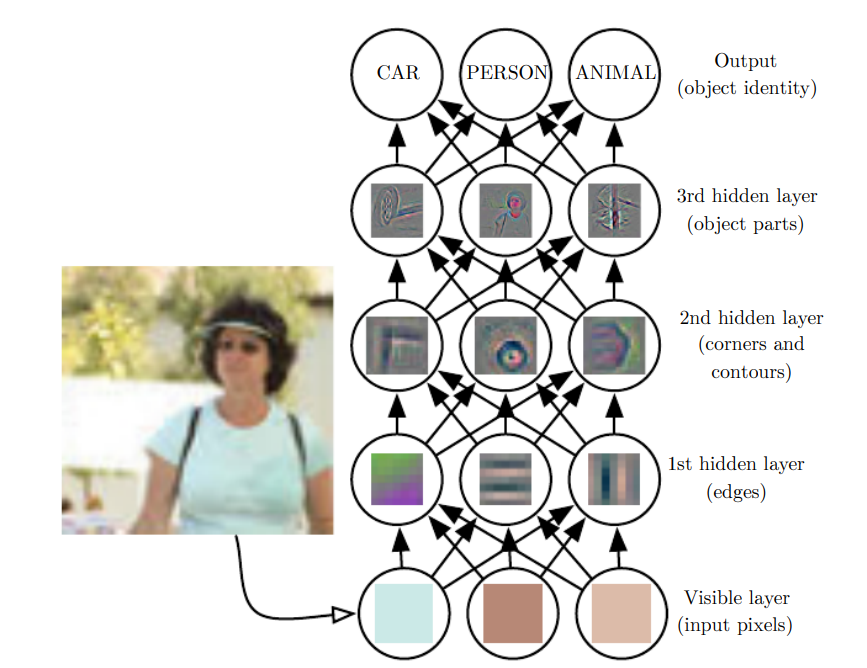
\includegraphics[width=\textwidth,height=0.8\textheight,keepaspectratio]{figures/Screenshot 2026-04-13 104137.png}
        \end{column}
    \end{columns}
\end{frame}

% ===== SLIDE 5: But What Did It Actually Learn? =====
\begin{frame}{But What Did It Actually Learn?}
    \begin{columns}[T]
        \begin{column}{0.62\textwidth}
            \begin{itemize}
                \vspace{0.3em}
                \item These models learn statistical patterns, not concepts.
                \vspace{0.3em}
                \item More layers means more complex features: from edges to shapes to objects, from words to phrases to meaning.
                \vspace{0.3em}
                \item Adding layers changes how the network thinks, not what it knows.
                \vspace{0.3em}
                \item Today: fine-tuning (changing how it thinks). Not RAG (changing what it knows).
                \vspace{0.3em}
                \item This is why LLMs hallucinate: they produce statistically plausible text, not verified facts.
            \end{itemize}
        \end{column}
        \begin{column}{0.35\textwidth}
            \textbf{Ribeiro et al.\ (2016):}\\
            A husky/wolf classifier was detecting snow in the background, not the animal.

                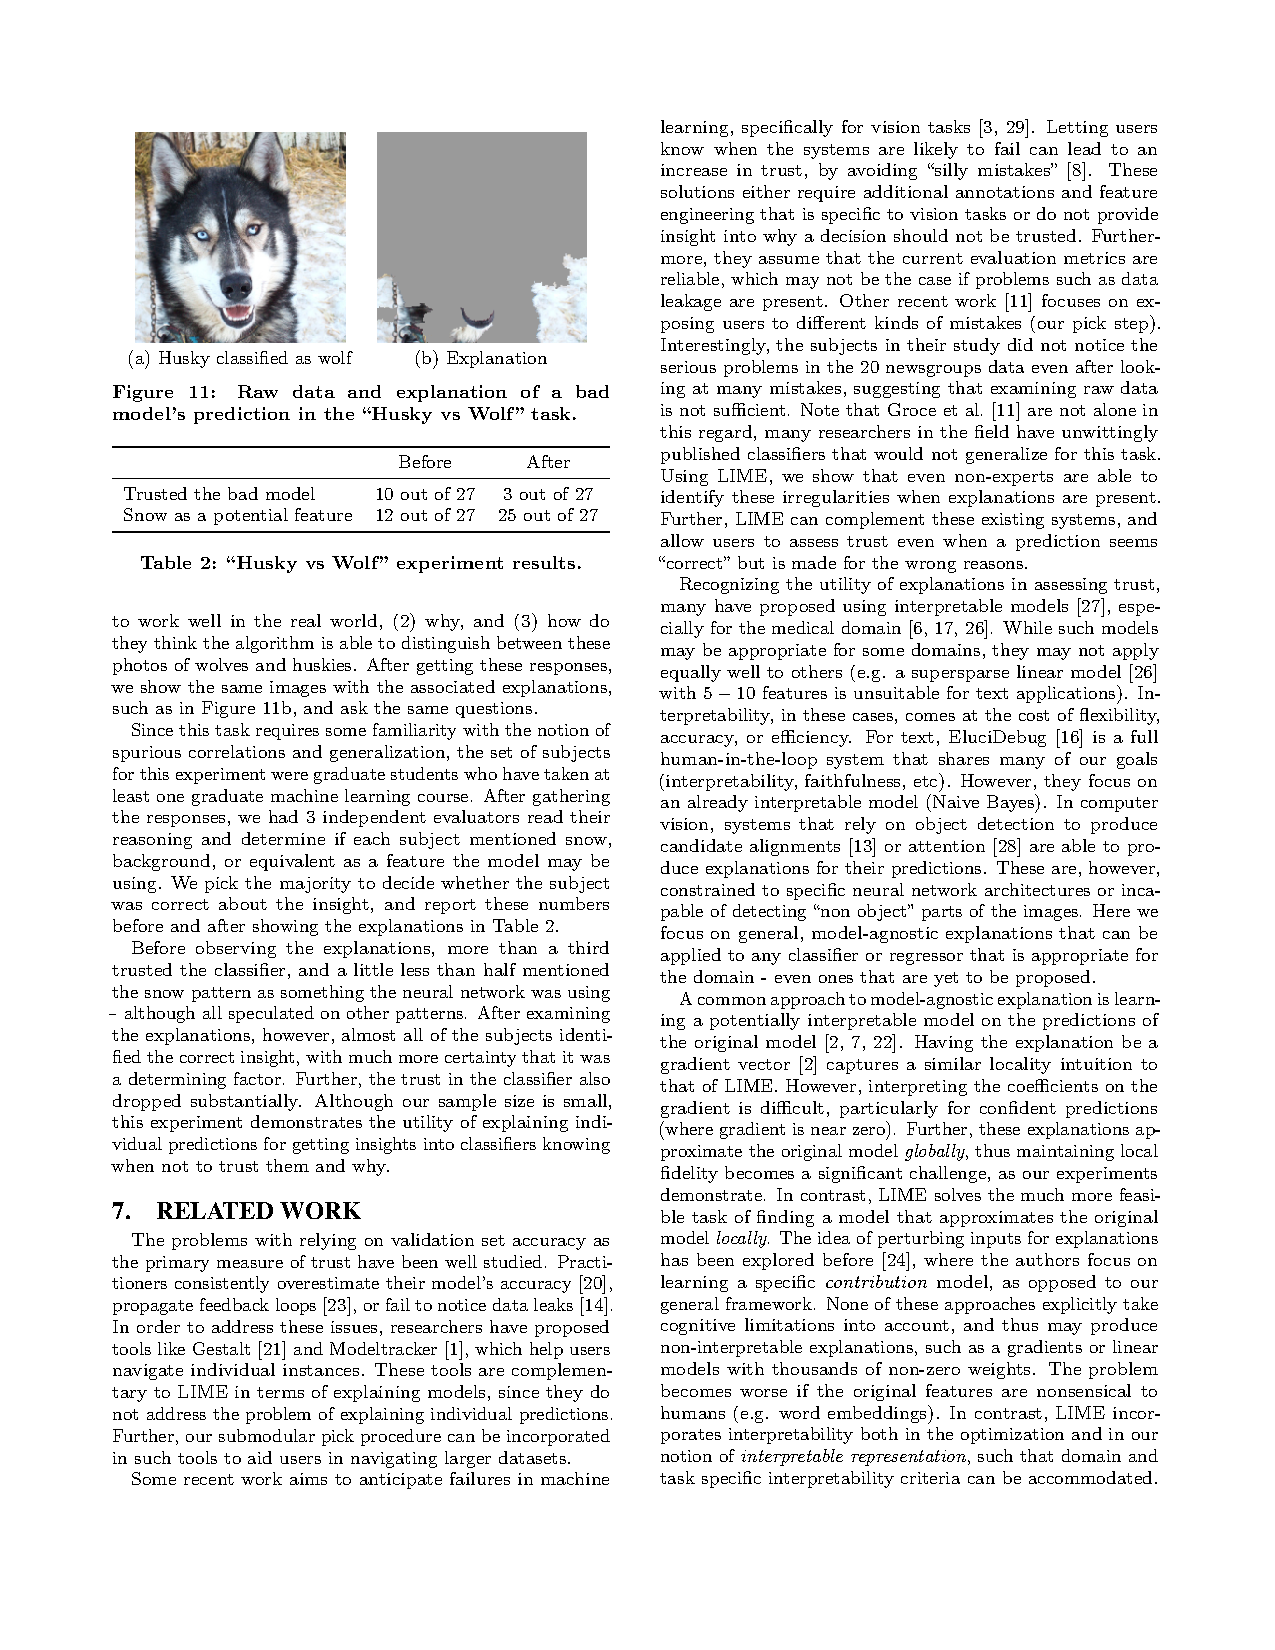
\includegraphics[width=1.1\textwidth,clip,trim=30 652 340 55,page=1]{figures/ribeiro2016_fig11_husky_wolf.pdf}\\
                {\scriptsize Fig.~11, \href{https://arxiv.org/abs/1602.04938}{arXiv:1602.04938}}
        \end{column}
    \end{columns}
\end{frame}

% ===== SLIDE 6: From Images to Language =====
\begin{frame}{From Images to Language}
    A Large Language Model (LLM) predicts the next word based on patterns learned from massive text data. Not a database, not a search engine: a pattern completer.

    \vspace{0.8em}
    \begin{center}
        ``The cat sat on the \underline{\hspace{2cm}}''

        \vspace{0.3em}
        \texttt{mat} (high probability) \hspace{2em} \texttt{quantum} (low probability)
    \end{center}

    \vspace{0.8em}
    \begin{table}
        \centering
        \begin{tabular}{llll}
            \toprule
            \textbf{Model} & \textbf{Parameters} & \textbf{File Size} & \textbf{RAM Needed} \\
            \midrule
            Llama 3.2 1B  & 1 billion  & $\sim$1.3 GB & $\sim$2 GB \\
            Llama 3.2 3B  & 3 billion  & $\sim$2.0 GB & $\sim$4 GB \\
            Llama 3.1 8B  & 8 billion  & $\sim$4.7 GB & $\sim$8 GB \\
            Llama 3.1 70B & 70 billion & $\sim$40 GB  & $\sim$48 GB \\
            \bottomrule
        \end{tabular}
    \end{table}
\end{frame}

% =============================================================================
% ACT 2: OLLAMA + WRITING DEMO (Slides 8-13)
% =============================================================================

% ===== SLIDE 8: It's Just a File =====
\begin{frame}[fragile]{It's Just a File}
    You can download an LLM and run it on your laptop: no internet, no account, no subscription.

    \vspace{0.8em}
    Ollama is a free, open-source app that downloads and runs LLMs on your machine.

    \vspace{0.8em}
    \textbf{Install:}
    \begin{lstlisting}
curl -fsSL https://ollama.com/install.sh | sh
    \end{lstlisting}
    \textbf{Windows:} Download from \href{https://ollama.com}{ollama.com}

    \vspace{0.8em}
    Supports models from Meta (Llama), Google (Gemma 4), Alibaba (Qwen 3), Microsoft (Phi-4), and more.
\end{frame}

% ===== SLIDE 9: What Can Ollama Do? =====
\begin{frame}{What Can Ollama Do?}
    It works like a browser LLM, but it can also be customized:
    \begin{itemize}
        \vspace{0.3em}
        \item \textbf{Cloud models:} some models are too large for your hardware. Ollama can run them on remote servers and send the results back to you.
        \vspace{0.3em}
        \item \textbf{Web search:} by default, models only know what they learned during training. Web search lets them look up current information before answering.
        \vspace{0.3em}
        \item \textbf{Context length:} controls how much text the model can ``see'' at once. A longer context lets you paste in entire papers, but uses more RAM.
        \vspace{0.3em}
        \item \textbf{Network access:} expose Ollama to your local network so other devices can connect to the same model. One powerful machine runs the model, everyone in the lab uses it.
    \end{itemize}
\end{frame}

% ===== SLIDE 10: AI for Writing =====
\begin{frame}{AI for Writing}
    AI as a writing companion, not a ghost writer. Three reasons not to let AI write for you:
    \begin{itemize}
        \vspace{0.3em}
        \item It hallucinates: plausible-sounding text that may be wrong.
        \vspace{0.3em}
        \item It has a distinctive style: readers (and reviewers) can tell.
        \vspace{0.3em}
        \item It dulls your thinking (\href{https://doi.org/10.3389/feduc.2026.1759062}{paper}) and impairs skill formation (\href{https://arxiv.org/abs/2601.20245}{paper}).
    \end{itemize}

    \vspace{0.8em}
    Instead, use it as a ping-pong partner, paragraph by paragraph:
    \begin{itemize}
        \vspace{0.3em}
        \item Have a few ideas but don't know how to connect them
        \vspace{0.3em}
        \item Want to avoid a repetitive word
        \vspace{0.3em}
        \item Want to reference a particular number, add a figure, or cite something
        \vspace{0.3em}
        \item Help review for consistency
    \end{itemize}
\end{frame}

% ===== SLIDE 11: Demo — Writing with AI =====
\begin{frame}{Demo: Writing with AI}
    \begin{userbox}
        \small
        I have these three ideas for a paragraph:\\
        1. The Hamiltonian is symmetric but the ground state is not\\
        2. This is called spontaneous symmetry breaking\\
        3. It explains why phase transitions happen\\[0.3em]
        Write a paragraph connecting these ideas. About 80 words, formal physics style.
    \end{userbox}

    \vspace{0.5em}
    \begin{assistantbox}
        \small
        ``Although the governing Hamiltonian respects the full symmetry of the system, the ground state spontaneously selects a preferred configuration, breaking this symmetry. This phenomenon, known as spontaneous symmetry breaking, provides a unifying framework for understanding phase transitions in condensed matter systems\ldots''
    \end{assistantbox}
\end{frame}

% ===== SLIDE 12: Demo — Ping-Pong =====
\begin{frame}{Demo: Ping-Pong}
    Now refine. You could say:
    \begin{itemize}
        \vspace{0.3em}
        \item ``Be less formal''
        \vspace{0.3em}
        \item ``This is too concise, expand the third point''
        \vspace{0.3em}
        \item ``Avoid the word `fundamental'\,''
        \vspace{0.3em}
        \item ``Start with the phase transition, not the Hamiltonian''
        \vspace{0.3em}
        \item ``Split this into two sentences''
    \end{itemize}

    \vspace{0.5em}
    \begin{assistantbox}
        \small
        ``Phase transitions in condensed matter arise from a striking asymmetry: while the Hamiltonian treats all configurations equally, the ground state does not. The system spontaneously selects a preferred direction, breaking the underlying symmetry\ldots''
    \end{assistantbox}
\end{frame}

% ===== SLIDE 13: Problem — It Forgot My Introduction =====
\begin{frame}{Problem: It Forgot My Introduction}
    Paragraph-by-paragraph assistance works great with small models that fit on virtually any modern laptop (e.g., Llama 3.2 3B, just 2 GB).

    \vspace{0.8em}
    But what if you want the model to reference something you wrote earlier in your paper? It can't. The model can only see $\sim$3 pages of text (4,096 tokens by default).

    \vspace{0.5em}
    \begin{itemize}
        \vspace{0.3em}
        \item It has no memory of your paper
        \vspace{0.3em}
        \item Only what's in the current conversation window
        \vspace{0.3em}
        \item Earlier context silently drops off
    \end{itemize}

    \vspace{1em}
    Can we fix this?
\end{frame}

% =============================================================================
% ACT 3: CONTEXT WINDOWS & QUANTIZATION (Slides 16-20)
% =============================================================================

% ===== SLIDE 14: What Is a Context Window? =====
\begin{frame}{What Is a Context Window?}
    A token is the fundamental unit of information for LLMs (roughly 3/4 of a word).

    \vspace{0.5em}
    The context window is the amount of text the model can ``see'' at once. Everything you send + everything it replies must fit in the window. Tradeoff: bigger context = more RAM.

    \vspace{0.5em}
    \begin{table}
        \centering
        \begin{tabular}{lll}
            \toprule
            \textbf{Context Size} & \textbf{Practical Use} & \textbf{RAM (3B model)} \\
            \midrule
            4K (default)  & Short conversations        & $\sim$3 GB \\
            16K           & A few pages of a paper      & $\sim$5 GB \\
            32K           & A full paper                & $\sim$7 GB \\
            128K          & Multiple papers             & $\sim$16 GB \\
            \bottomrule
        \end{tabular}
    \end{table}

    \vspace{0.3em}
    Rule of thumb: 16K--32K is practical for most laptops.
\end{frame}


% ===== SLIDE 15: Quantization =====
\begin{frame}{Quantization: Making Models Fit}
    Full-precision models are huge: a 7B model is $\sim$14 GB. Quantization rounds the numbers to use fewer bits, like JPEG compression for AI. Smaller file, slight quality loss.

    \vspace{0.5em}
    The RAM you save can be used for a larger context window.

    \vspace{0.5em}
    \begin{table}
        \centering
        \begin{tabular}{lll}
            \toprule
            \textbf{Level} & \textbf{Bits/Param} & \textbf{Quality} \\
            \midrule
            FP16 (full)  & 16 bits & Original \\
            Q8            & 8 bits  & Near-original \\
            Q4            & 4 bits  & Good balance \\
            Q2            & 2 bits  & Very compressed, noticeable loss \\
            \bottomrule
        \end{tabular}
    \end{table}

    \vspace{0.3em}
    This is why a 3B model fits in 2 GB instead of 6 GB. Models on Ollama's library come pre-quantized (usually Q4). No action needed.
\end{frame}

% ===== SLIDE 16: Demo — Full Paper in Context =====
\begin{frame}{Demo: Full Paper in Context}
    With a larger context window, you can paste an entire paper into the conversation and ask questions about it:

    \begin{itemize}
        \vspace{0.3em}
        \item ``Summarize the main argument in 2 sentences''
        \vspace{0.3em}
        \item ``Is the notation in Section 3 consistent with Section 2?''
        \vspace{0.3em}
        \item ``Does the conclusion follow from the results?''
    \end{itemize}

    \vspace{0.8em}
    The model gives substantive answers referencing specific sections. It can proofread and check your paper for consistency.

    \vspace{0.5em}
    \begin{tcolorbox}[colback=gray!10, colframe=gray!40, boxrule=0.5pt, arc=2pt, fontupper=\small]
        Demo: paste \texttt{sample\_paper.txt} into Ollama with 32K context
    \end{tcolorbox}
\end{frame}

% ===== SLIDE 17: What's Still Missing =====
\begin{frame}{What's Still Missing}
    But ask it to write like your field, and you get generic text. ``Magnetic frustration is a fascinating phenomenon\ldots'' sounds like a blog post, not a physics paper.

    \vspace{0.8em}
    It doesn't know:
    \begin{itemize}
        \vspace{0.3em}
        \item What notation is standard in your subfield
        \vspace{0.3em}
        \item What a typical abstract sounds like
        \vspace{0.3em}
        \item What methods or terminology reviewers expect
    \end{itemize}

    \vspace{1em}
    It's helpful, but not specialized. What if we could teach it?
\end{frame}

% =============================================================================
% ACT 4: FINE-TUNING WITH LoRA (Slides 21-26)
% =============================================================================

% ===== SLIDE 18: What Is Fine-Tuning? =====
\begin{frame}{What Is Fine-Tuning?}
    Remember: adding layers changes how the network thinks, not what it knows.

    \vspace{0.5em}
    Fine-tuning adds small new layers to a pre-trained model and trains them on your data. The original model stays frozen. The new layers learn to adjust how it thinks: writing style, terminology, conventions.

    \begin{itemize}
        \vspace{0.3em}
        \item Pre-training: done by Meta, Google, etc. Costs millions. Trains on the entire internet.
        \vspace{0.3em}
        \item Fine-tuning: done by you. Costs hours. Trains on your field's papers.
    \end{itemize}

    \vspace{0.5em}
    In Session 6, we saw Chemma: a 7B model fine-tuned on 1.28M chemistry Q\&A pairs that outperformed GPT-4 at optimizing a novel reaction (\href{https://arxiv.org/abs/2504.18340}{Zhang et al., 2025}).

    \vspace{0.5em}
    The result: a model that thinks like a domain expert, not a generalist.
\end{frame}

% ===== SLIDE 22: LoRA =====
\begin{frame}{LoRA: The Trick That Makes It Possible}
    \begin{columns}[T]
        \begin{column}{0.48\textwidth}
            \textbf{Full Fine-Tuning}

            \vspace{0.5em}
            \begin{tcolorbox}[colback=red!5, colframe=red!40, boxrule=0.5pt, arc=2pt]
                Update all 3 billion parameters

                \vspace{0.3em}
                {\small
                \begin{itemize}
                    \item Needs huge GPU
                    \item Tons of data required
                    \item Produces a full copy of the model
                \end{itemize}
                }
            \end{tcolorbox}
        \end{column}
        \begin{column}{0.48\textwidth}
            \textbf{LoRA (Low-Rank Adaptation)}

            \vspace{0.5em}
            \begin{tcolorbox}[colback=green!5, colframe=green!40, boxrule=0.5pt, arc=2pt]
                Freeze original, add small trainable layers

                \vspace{0.3em}
                {\small
                \begin{itemize}
                    \item Train $\sim$1--10M new parameters
                    \item Adapter file: $\sim$50--100 MB
                    \item Fits on a single GPU
                \end{itemize}
                }
            \end{tcolorbox}
        \end{column}
    \end{columns}

    \vspace{1em}
    \textbf{QLoRA:} Same idea + quantize the base model $\rightarrow$ even less memory.

    \vspace{0.5em}
    Analogy: adding sticky notes on a textbook.
\end{frame}

% ===== SLIDE 23: Training Data =====
\begin{frame}{Training Data: arXiv Papers}
    \textbf{Goal:} Teach the model the conventions of a physics subfield --- in our case, \texttt{cond-mat.str-el} (strongly correlated electrons).

    \vspace{0.5em}
    \textbf{Source:} 100 recent papers (Oct 2025 -- Mar 2026) from \href{https://arxiv.org}{arXiv}. Full LaTeX source, not just abstracts.

    \vspace{0.5em}
    \textbf{Turning 100 papers into 2{,}282 training examples.} From each paper we extract four kinds of prompt $\rightarrow$ completion pairs:
    \begin{itemize}
        \vspace{0.2em}
        \item \textit{Title $\rightarrow$ abstract} --- what should this paper emphasize?
        \item \textit{Intro paragraph $\rightarrow$ continuation} --- flow and coherence.
        \item \textit{Section heading + context $\rightarrow$ section body} --- structure and argument.
        \item \textit{Paper body $\rightarrow$ abstract} --- summarization in the field's voice.
    \end{itemize}

    \vspace{0.3em}
    One paper $\approx$ 25 examples. 100 papers $\rightarrow$ 2{,}282 train + 254 validation.

    \vspace{0.5em}
    The model doesn't need a million papers --- LoRA only adjusts a few million parameters. A few thousand high-quality examples is plenty.
\end{frame}

% ===== SLIDE 24: Running on NRP JupyterHub =====
\begin{frame}{Accessing NRP}
    \hypertarget{nrp-access}{}
    The National Research Platform (NRP) is a free, NSF-funded GPU compute platform shared across US universities, including Berkeley.

    \vspace{0.5em}
    \textbf{Get access:} Create a portal account with CalNet, then request a namespace in the Nautilus Support room on Matrix. Approval typically takes hours.

    \vspace{0.5em}
    \textbf{What you get:} A JupyterHub interface at \href{https://jupyterhub-west.nrp-nautilus.io}{\texttt{jupyterhub-west.nrp-nautilus.io}} with GPUs (A100, H100, RTX-series) and a ``Deep Learning'' image that ships with PyTorch + transformers preinstalled.

    \vspace{0.5em}
    \begin{tcolorbox}[colback=red!5, colframe=red!40, boxrule=0.5pt, arc=2pt, fontupper=\small]
        \textbf{Warning --- Pod Reclamation:} NRP is a shared cluster. Your JupyterHub pod can be killed without warning if a higher-priority job needs the GPU. Our training took 3 attempts before finishing!\\[0.3em]
        \textbf{Protect yourself:} save checkpoints frequently and back up outputs immediately.
    \end{tcolorbox}

    \vspace{0.3em}
    \hfill\hyperlink{nrp-onboarding}{\beamergotobutton{Onboarding details}}
\end{frame}

% ===== SLIDE 24b: Training a LoRA Adapter =====
\begin{frame}{Training a LoRA Adapter}
    The Hugging Face ecosystem handles the heavy lifting. At a high level:

    \vspace{0.5em}
    Load a pretrained model in 4-bit $\rightarrow$ attach a small LoRA adapter $\rightarrow$ train on your data $\rightarrow$ save the adapter ($\sim$100 MB).

    \vspace{0.5em}
    That's $\sim$50 lines of Python. You don't need to understand every hyperparameter to get started.

    \vspace{0.7em}
    \textbf{Tutorials to learn from:}
    \begin{itemize}
        \vspace{0.2em}
        \item \href{https://huggingface.co/docs/peft}{Hugging Face PEFT docs} --- the canonical reference
        \item \href{https://github.com/mlabonne/llm-course}{Maxime Labonne's LLM Course} --- free, hands-on notebooks
        \item \href{https://www.philschmid.de/fine-tune-llms-in-2024-with-trl}{Philipp Schmid's QLoRA walkthrough} --- single blog post, very clear
    \end{itemize}

    \vspace{0.7em}
    \textbf{Where it runs:} Any CUDA GPU with $\sim$12 GB VRAM --- NRP, Savio, Colab, or a laptop. Our notebook is in the workshop repo.
\end{frame}

% ===== SLIDE 24c: What to Train On, What to Train =====
\begin{frame}{Where Will You Run It? \& Prior Art in Science}
    \textbf{Where will you run it?} Pick a base model that fits the hardware.
    \begin{itemize}
        \vspace{0.2em}
        \item \textbf{Laptop} ($\leq$16 GB RAM): 1B--3B parameters. Qwen 2.5 3B, Llama 3.2 3B, Gemma 3 4B.
        \item \textbf{Workstation or one GPU:} 7B--8B. Llama 3.1 8B, Qwen 2.5 7B.
        \item \textbf{Shared cluster} (NRP, Savio): 13B--70B when you need the extra capability.
    \end{itemize}

    \vspace{0.6em}
    \textbf{Successful scientific fine-tunes to learn from:}
    \begin{itemize}
        \vspace{0.2em}
        \item \href{https://arxiv.org/abs/2311.16079}{\textbf{Meditron-70B}} (EPFL, 2023): Llama 2 fine-tuned on PubMed + medical guidelines. Matches GPT-3.5 on clinical benchmarks.
        \item \href{https://arxiv.org/abs/2210.10341}{\textbf{BioGPT}} (Microsoft, 2022): GPT-2 fine-tuned on 15M PubMed abstracts. Strong at biomedical relation extraction.
        \item \href{https://arxiv.org/abs/2303.17564}{\textbf{BloombergGPT}} (2023): 50B-parameter model trained on 363B tokens of financial text. Domain outperforms general LLMs on finance tasks.
        \item \href{https://arxiv.org/abs/2504.18340}{\textbf{Chemma}} (Zhang et al., 2025): 7B fine-tuned on 1.28M chemistry Q\&A pairs. Beat GPT-4 at reaction optimization.
    \end{itemize}
\end{frame}

% ===== SLIDE 25: Demo 3a — Base vs. Fine-Tuned =====
\begin{frame}{Demo 3a: Base Model vs.\ Fine-Tuned Model}
    \textbf{Prompt:} ``Write an abstract for a paper titled: \emph{Pressure-induced superconductivity in the kagome metal CsV$_3$Sb$_5$}.''

    \vspace{0.4em}
    \begin{columns}[T]
        \begin{column}{0.48\textwidth}
            \textbf{Base Model}
            \begin{tcolorbox}[colback=gray!10, colframe=gray!40, boxrule=0.5pt, arc=2pt, fontupper=\footnotesize]
                ``The discovery of pressure-induced superconductivity in the kagome metal CsV$_3$Sb$_5$ represents a significant advance in the field of unconventional superconductors. This study investigates the effect of hydrostatic pressure on the electronic and magnetic properties\ldots''
            \end{tcolorbox}
            {\footnotesize\color{red} Review-paper opener; vague ``represents a significant advance.''}
        \end{column}
        \begin{column}{0.48\textwidth}
            \textbf{Fine-Tuned Model}
            \begin{tcolorbox}[colback=blue!5, colframe=blue!30, boxrule=0.5pt, arc=2pt, fontupper=\footnotesize]
                ``The kagome compound CsV$_3$Sb$_5$ is reported to exhibit superconductivity at 12~K under high pressure. Here we report that this originates from a direct band crossing of the V-$d_{x^2-y^2}$ orbital, supported by first-principles calculations\ldots''
            \end{tcolorbox}
            {\footnotesize\color{green!50!black} Specific mechanism, orbital notation, ``Here we report\ldots''}
        \end{column}
    \end{columns}
\end{frame}

% ===== SLIDE 26: Demo 3b — Field-Specific Questions =====
\begin{frame}{Demo 3b: Writing in the Field's Voice}
    \textbf{Prompt:} ``Continue this paragraph from a condensed matter physics paper: \emph{The interplay between strong electron correlations and spin-orbit coupling has emerged as a central theme in the study of 4d and 5d transition metal oxides. In these systems,}\ldots''

    \vspace{0.4em}
    \begin{columns}[T]
        \begin{column}{0.48\textwidth}
            \textbf{Base Model}
            \begin{tcolorbox}[colback=gray!10, colframe=gray!40, boxrule=0.5pt, arc=2pt, fontupper=\footnotesize]
                ``\ldots the unique combination of these effects leads to fascinating phenomena such as unconventional superconductivity, topological insulators, and quantum spin liquids. Understanding these interactions is crucial for unraveling\ldots''
            \end{tcolorbox}
            {\footnotesize\color{red} Lists buzzwords; reads like a review.}
        \end{column}
        \begin{column}{0.48\textwidth}
            \textbf{Fine-Tuned Model}
            \begin{tcolorbox}[colback=blue!5, colframe=blue!30, boxrule=0.5pt, arc=2pt, fontupper=\footnotesize]
                ``\ldots the strong SOC induces nontrivial Berry curvature for both itinerant electrons and localized moments, leading to a complex energy spectrum and enhanced many-body effects~[citation]. While much progress has been made\ldots, the full phase diagram \ldots remains largely uncharted.''
            \end{tcolorbox}
            {\footnotesize\color{green!50!black} Specific mechanism, \texttt{[citation]} placeholder, hedged claim.}
        \end{column}
    \end{columns}

    \vspace{0.3em}
    {\footnotesize\textbf{Caveat:} it learned \textit{statistical patterns}, not ground truth --- always verify.}
\end{frame}

% =============================================================================
% ACT 5: HUGGING FACE & DEPLOYMENT (Slides 27-30)
% =============================================================================

% ===== SLIDE 27: From NRP to the World =====
\begin{frame}[fragile]{From NRP to the World}
    You trained a model. It lives on an NRP node. Now what?

    \vspace{0.6em}
    \href{https://huggingface.co}{Hugging Face} = GitHub for AI models. Upload the adapter ($\sim$130 MB) once, anyone can pull it down.

    \vspace{0.5em}
    \begin{lstlisting}[language=bash]
hf auth login --token $HF_TOKEN
hf upload brunosmaniotto/condmat-qwen25-qlora-fullpapers \
    ./physics-adapter-fullpapers . --repo-type=model
    \end{lstlisting}

    \vspace{0.4em}
    \textbf{Our adapter is live:} \href{https://huggingface.co/brunosmaniotto/condmat-qwen25-qlora-fullpapers}{\texttt{hf.co/brunosmaniotto/condmat-qwen25-qlora-fullpapers}}

    \vspace{0.6em}
    \textbf{A good model card includes:}
    \begin{itemize}
        \item Intended use and limitations
        \item Load snippet (so people can actually run it)
        \item Training data, hyperparameters, hardware
        \item License of the base model you built on
    \end{itemize}
\end{frame}

% ===== SLIDE 28: Deployment Options =====
\begin{frame}{Deployment Options}
    \begin{table}
        \centering
        \begin{tabular}{@{}p{0.30\textwidth}p{0.28\textwidth}p{0.36\textwidth}@{}}
            \toprule
            \textbf{Option} & \textbf{Cost} & \textbf{Best For} \\
            \midrule
            \textbf{Ollama on your laptop} & Free & Personal use, privacy \\
            \addlinespace
            \textbf{Google Colab} & Free (Pro via Berkeley) & Interactive, faster GPU \\
            \addlinespace
            \textbf{Kaggle Notebooks} & Free (30 hrs/wk GPU) & Reproducible workflows \\
            \addlinespace
            \textbf{Hugging Face Spaces} & Free (ZeroGPU) & Shareable demo apps \\
            \bottomrule
        \end{tabular}
    \end{table}

    \vspace{0.5em}
    \textbf{Key:} Berkeley provides Colab Pro for free --- gives you T4/V100 GPUs and longer runtimes.

    \vspace{0.5em}
    For most researchers: start with Ollama locally, use Colab for collaboration.
\end{frame}

% ===== SLIDE 26: When to Fine-Tune vs. When to Just Prompt =====
\begin{frame}{When to Fine-Tune vs.\ When to Just Prompt}
    A useful distinction: does your task need complex instructions, or complex thinking?

    \begin{itemize}
        \vspace{0.3em}
        \item Complex instructions (prompt engineering): ``write this paragraph in formal style, avoid passive voice, use these three terms.'' The model already knows how. You just need to tell it what you want.
        \vspace{0.3em}
        \item Complex thinking (fine-tuning): ``write like a condensed matter physicist.'' The model doesn't know how. You need to change how it thinks.
    \end{itemize}

    \vspace{0.5em}
    \begin{table}
        \centering
        \small
        \begin{tabular}{lll}
            \toprule
            & \textbf{Prompt Engineering} & \textbf{Fine-Tuning} \\
            \midrule
            What it does & Steers a generalist with instructions & Changes how the model thinks \\
            Example & ``Rewrite this more formally'' & Training on 100 full arXiv papers \\
            Effort & Zero setup & Hours of training, needs GPU \\
            Data stays & With the provider (unless local) & Local, the adapter is yours \\
            \bottomrule
        \end{tabular}
    \end{table}
\end{frame}

% ===== SLIDE 30b: RAG vs. Fine-Tuning =====
\begin{frame}{RAG vs.\ Fine-Tuning: Information vs.\ Thinking}
    \begin{columns}[T]
        \begin{column}{0.48\textwidth}
            RAG (Retrieval-Augmented Generation)

            \vspace{0.4em}
            Gives the model new information.

            \vspace{0.5em}
            \begin{itemize}
                \item Fetches relevant documents at query time
                \item Model reads them as context, then answers
                \item Great for: facts, policies, recent data, specific documents
            \end{itemize}
        \end{column}
        \begin{column}{0.48\textwidth}
            Fine-Tuning (LoRA / QLoRA)

            \vspace{0.4em}
            Changes how the model thinks.

            \vspace{0.5em}
            \begin{itemize}
                \item Modifies the model's weights permanently
                \item Model internalizes style, conventions, reasoning patterns
                \item Great for: tone, domain style, specialized writing, field conventions
            \end{itemize}
        \end{column}
    \end{columns}

    \vspace{1em}
    Use RAG when you need the model to know specific things. Use fine-tuning when you need it to write or reason like a domain expert. They can also be combined.
\end{frame}

% ===== CLOSING =====
\begin{frame}[plain]
    \vfill
    \begin{center}
        {\Large Questions?}
    \end{center}
    \vfill
\end{frame}

% =============================================================================
% APPENDIX
% =============================================================================
\appendix

\begin{frame}{Appendix: How We Onboarded to NRP}
    \hypertarget{nrp-onboarding}{}

    \textbf{1. Create a portal account} at \href{https://portal.nrp-nautilus.io}{portal.nrp-nautilus.io} using CalNet (CILogon).

    \vspace{0.4em}
    \textbf{2. Request a namespace} by posting in the \textbf{Nautilus Support} room on Matrix (via the Element client). The admin team reviews requests directly.

    \vspace{0.4em}
    \textbf{3. The message we sent:}
    \begin{tcolorbox}[colback=gray!8, colframe=gray!40, boxrule=0.5pt, arc=2pt, fontupper=\small]
        \itshape
        Hi, I'm a researcher at UC Berkeley (D-Lab). I'd like to request a new namespace for running AI/ML workshops --- specifically for fine-tuning open-weight LLMs with LoRA as part of a teaching series. My portal account is \texttt{brunosmaniotto@berkeley.edu}. Could I be promoted to namespace admin? Suggested namespace name: \texttt{berkeley-dlab}. Thank you!
    \end{tcolorbox}

    \vspace{0.3em}
    \textbf{4. Wait for approval.} Ours was approved within hours.

    \vspace{0.4em}
    \textbf{5. Log in} at \href{https://jupyterhub-west.nrp-nautilus.io}{\texttt{jupyterhub-west.nrp-nautilus.io}} with CalNet, launch a server with the \textit{NRP Deep Learning} image and a GPU.

    \vspace{0.5em}
    \hfill\hyperlink{nrp-access}{\beamerreturnbutton{Back to Accessing NRP}}
\end{frame}

\end{document}
